\documentclass[11pt,a4paper]{article}
\usepackage[margin=23mm,headheight=15pt]{geometry}
\usepackage[T1]{fontenc}
\usepackage{tgpagella}
\usepackage{amsmath,amssymb,amsthm,mathtools,bm}
\usepackage{microtype,booktabs,tabularx,array,enumitem,multicol}
\usepackage{tikz}
\usetikzlibrary{arrows.meta,positioning,calc,decorations.pathmorphing}
\usepackage{fancyhdr,xcolor,hyperref}
\definecolor{deepblue}{RGB}{25,50,99}
\definecolor{purple}{RGB}{104,69,170}
\definecolor{softblue}{RGB}{225,237,251}
\hypersetup{colorlinks=true,urlcolor=deepblue,linkcolor=deepblue}
\pagestyle{fancy}\fancyhf{}\fancyhead[L]{\small Quantum Coherence and Matter-Wave Interference}\fancyhead[R]{\small Physics Companion II}\fancyfoot[C]{\thepage}
\setlength{\parskip}{5pt}\setlength{\parindent}{0pt}
\emergencystretch=2em
\setcounter{secnumdepth}{3}
\newtheorem{example}{Worked Example}
\newtheorem{remark}{Remark}
\newcommand{\Rb}{^{87}\mathrm{Rb}}
\newcommand{\kb}{k_{\mathrm B}}
\newcommand{\dd}{\mathrm d}
\newcommand{\ii}{\mathrm i}
\newcommand{\hc}{\hbar}
\begin{document}
\begin{center}
{\Large\bfseries\color{deepblue} Quantum Coherence, Matter-Wave Interference\\ and the Measurement of Bose--Einstein Condensates}\par\medskip
{\large Rubidium-87: From a Common Orbital to an Experimental Signal}\\[5pt]
{\small 17 November 2026 \quad $\cdot$ \quad Extended companion chapter \quad $\cdot$ \quad 14 worked examples}
\end{center}
\begin{abstract}
A Bose--Einstein condensate exhibits macroscopic occupation of a motional quantum state, but quantum coherence is not a photograph of 20,000 atoms occupying a single visible object. This companion chapter develops the quantitative bridge from the condensate order parameter to observable interference, first- and second-order correlation functions, time-of-flight imaging, release energies, free expansion, interactions, vortex phase winding, and atom interferometry. A separate case study describes the November 2026 optical-dipole-trap experiment aboard China's Tiangong space station and carefully distinguishes its 9.7-pK \emph{equivalent expansion temperature} from equilibrium thermometry. Every numerical example states its assumptions; no illustrative model curve is represented as an experimental data reconstruction.
\end{abstract}
\tableofcontents\newpage

\section{Three questions that a condensate experiment must answer}
A gas of $\Rb$ atoms becomes a Bose--Einstein condensate when one natural orbital of its one-body density matrix is macroscopically occupied. This concerns the motion of \emph{whole atoms}; the individual atoms retain their internal electronic states. Three measurable questions are distinct: (i) how many atoms are condensed? (ii) how spatially coherent is the sample? and (iii) how small is its kinetic or expansion energy? A condensate fraction, a coherence length and an equivalent expansion temperature need not be interchangeable quantities.

In a useful symmetry-broken mean-field description, a condensate is represented by
\begin{equation}\Psi(\mathbf r,t)=\sqrt{n_c(\mathbf r,t)}\,e^{\ii\theta(\mathbf r,t)},\qquad \int|\Psi|^2\dd^3r=N_0.\label{eq:order}\end{equation}
The density $n_c=|\Psi|^2$ is readily associated with atom-counting images. The phase $\theta$ is detected by comparing coherent amplitudes rather than by measuring an absolute global phase. A fixed-number condensate can display first-order coherence without having a nonzero $\langle\hat\psi\rangle$ in a number-conserving description.

\begin{center}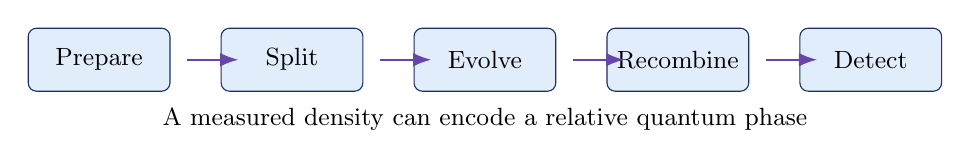
\begin{tikzpicture}[>=Latex,font=\small]
\foreach \x/\t in {0/Prepare,2.45/Split,4.9/Evolve,7.35/Recombine,9.8/Detect}{\node[draw=deepblue,rounded corners=3pt,fill=softblue,minimum width=1.8cm,minimum height=.8cm] at (\x,0) {\t};}
\foreach \x in {1.12,3.57,6.02,8.47}{\draw[->,thick,purple] (\x,0)--++(.65,0);}
\node[align=center] at (4.9,-.75) {A measured density can encode a relative quantum phase};
\end{tikzpicture}\end{center}

\section{Interference from the superposition principle}
\subsection{Two complex matter-wave amplitudes}
Let two phase-coherent components be $\Psi_A=\sqrt{n_A}e^{\ii\theta_A}$ and $\Psi_B=\sqrt{n_B}e^{\ii\theta_B}$. Upon overlap, the measured density is
\begin{align}
n(\mathbf r)&=|\Psi_A+\Psi_B|^2\\
&=n_A+n_B+2\sqrt{n_An_B}\cos(\theta_B-\theta_A).\label{eq:interference}
\end{align}
The interference term is physical: equal local densities and relative phases of zero or $\pi$ give constructive or destructive interference, respectively. A single density image, however, cannot in general determine arbitrary spatial phases without a reference, model or multiple measurements.

\begin{center}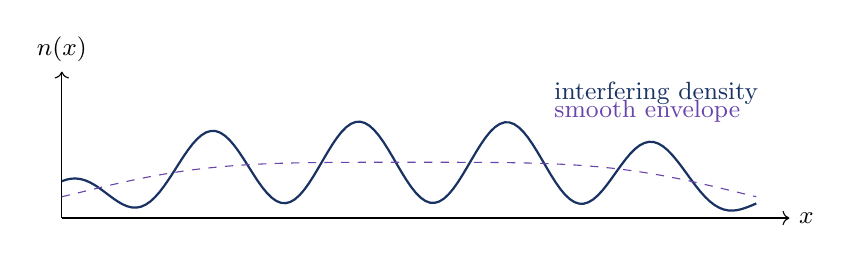
\begin{tikzpicture}[x=.84cm,y=.6cm,font=\small]
\draw[->] (0,0)--(11,0) node[right] {$x$};\draw[->] (0,0)--(0,3.1) node[above] {$n(x)$};
\draw[deepblue,thick,domain=0:10.5,samples=150] plot (\x,{1.18*(1+0.73*cos(deg(2.8*\x))) *exp(-((\x-5.25)/5.3)^4)});
\draw[purple,dashed,domain=0:10.5,samples=100] plot (\x,{1.18*exp(-((\x-5.25)/5.3)^4)});
\node[anchor=west,deepblue] at (7.3,2.65) {interfering density};
\node[anchor=west,purple] at (7.3,2.25) {smooth envelope};
\end{tikzpicture}\end{center}

\subsection{Fringe visibility}
An experimentally useful quantity is the local visibility or contrast
\begin{equation}\mathcal V=\frac{n_{\max}-n_{\min}}{n_{\max}+n_{\min}}.\label{eq:visibility}\end{equation}
For two perfectly phase-coherent components with equal density, $\mathcal V=1$ in the ideal model. If the densities are unequal, the maximal ideal visibility is $2\sqrt{n_An_B}/(n_A+n_B)$; detector resolution, shot averaging, multimode populations and phase noise can reduce it further. In particular, absence of fringes in an average image is not sufficient proof that individual experimental shots lacked coherence: independently prepared condensates can have shot-to-shot random relative phases.

\begin{example}[Visibility from a measured intensity range]
Suppose an atom-density line profile has peak $n_{\max}=180$ and trough $n_{\min}=60$ in the same calibrated units. Then $\mathcal V=(180-60)/(180+60)=0.50$. This is a measured contrast, not directly a 50\% condensate fraction.
\end{example}

\begin{example}[Unequal wave amplitudes]
For $n_A=9n_B$, even perfect mutual coherence yields $\mathcal V_{\rm ideal}=2\sqrt9/(9+1)=0.60$. A reduced contrast can therefore arise from simple imbalance rather than decoherence.
\end{example}

\section{Two expanding condensates and the fringe-spacing law}
\subsection{Free propagator and relative phase}
The nonrelativistic one-dimensional free propagator is
\begin{equation}
K(x,t;x',0)=\sqrt{\frac{M}{2\pi\ii\hc t}}\exp\!\left[\frac{\ii M(x-x')^2}{2\hc t}\right].
\end{equation}
For two initially localized packets centered at $x_A=-d/2$ and $x_B=+d/2$, the relative quadratic propagation phase in a sufficiently far-field region is
\begin{equation}
\Delta\theta(x,t)\simeq\frac{Mdx}{\hc t}+\theta_0.
\end{equation}
The density fringes consequently have period
\begin{equation}\boxed{\Lambda=\frac{ht}{Md}.}\label{eq:spacing}\end{equation}
The formula assumes coherent overlap, sufficiently simple free propagation, and negligible interaction-driven phase distortion during observation; it is not a universal fit to every BEC expansion image.

\begin{center}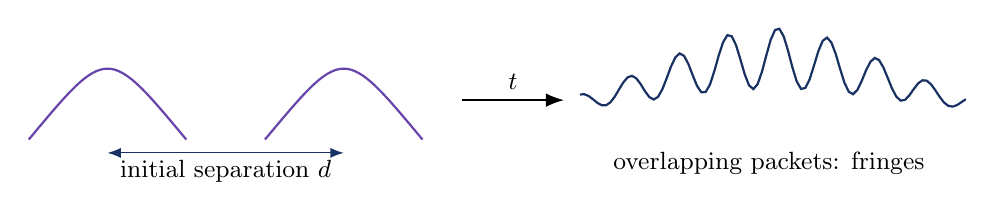
\begin{tikzpicture}[>=Latex,font=\small]
\draw[thick,purple] (0,0) .. controls (1,1.2) and (1,1.2) .. (2,0);
\draw[thick,purple] (3,0) .. controls (4,1.2) and (4,1.2) .. (5,0);
\node at (2.5,-.4) {initial separation $d$};
\draw[<->,deepblue] (1,-.17)--(4,-.17);
\draw[->,thick] (5.5,.5)--(6.8,.5) node[midway,above] {$t$};
\draw[thick,deepblue,domain=7:11.9,samples=90] plot (\x,{.33+.7*exp(-((\x-9.45)/2)^2)*(1+.55*cos(deg(10*(\x-7))))});
\node[align=center] at (9.4,-.3) {overlapping packets: fringes};
\end{tikzpicture}\end{center}

\begin{example}[Rubidium fringe spacing after 50 ms]
Use $M=1.443\times10^{-25}$ kg, $d=20\,\mu$m and $t=0.050$ s. Then
\[\Lambda=\frac{(6.62607015\times10^{-34})(0.050)}{(1.443\times10^{-25})(20\times10^{-6})}\simeq 11.48\,\mu\mathrm m.\]
The initially unobservable phase relation becomes a micrometre-scale spatial pattern.
\end{example}

\begin{example}[Recovering initial separation]
An image taken after $t=80$ ms has fringe period $\Lambda=15\,\mu$m. In the same far-field model, the initial separation was $d=ht/(M\Lambda)\simeq24.5\,\mu$m. A finite-resolution correction may be needed before interpreting an actual measured $\Lambda$.
\end{example}

\section{First- and second-order coherence}
\subsection{One-body density matrix}
In a general many-body system the first-order correlation function is
\begin{equation}
G^{(1)}(\mathbf r,\mathbf r')=\langle\hat\psi^\dagger(\mathbf r)\hat\psi(\mathbf r')\rangle,
\end{equation}
with normalized form
\begin{equation}
g^{(1)}(\mathbf r,\mathbf r')=\frac{G^{(1)}(\mathbf r,\mathbf r')}{\sqrt{n(\mathbf r)n(\mathbf r')}}.
\end{equation}
A pure fully condensed ideal state gives $G^{(1)}=N_0\phi_0^*(\mathbf r)\phi_0(\mathbf r')$. Long-range first-order coherence is the basis for interference visibility, subject to the geometry of the measurement. The Penrose--Onsager criterion defines condensation through an eigenvalue $N_0$ of this one-body density matrix that scales macroscopically with total atom number.

\subsection{Second-order coherence and shot noise}
The normally ordered second-order function is
\begin{equation}
G^{(2)}(\mathbf r,\mathbf r')=\langle\hat\psi^\dagger(\mathbf r)\hat\psi^\dagger(\mathbf r')\hat\psi(\mathbf r')\hat\psi(\mathbf r)\rangle.
\end{equation}
It probes density correlations and is logically distinct from phase coherence. For a single ideal mode of fixed occupation $N$,
\begin{equation}g^{(2)}(0)=\frac{N(N-1)}{N^2}=1-\frac1N,\end{equation}
whereas an ideal chaotic thermal mode gives $g^{(2)}(0)=2$. These statements assume idealized number statistics and appropriate detection conditions; a multimode gas and finite detector resolution require more care.

\begin{example}[Finite-$N$ second-order coherence]
For $N=20,000$ bosons in an ideal single-mode number state, $g^{(2)}(0)=1-1/20000=0.99995$. The numerical closeness to unity does not by itself prove perfect spatial coherence or quantify temperature.
\end{example}

\section{The superfluid velocity and a quantized vortex}
Write $\Psi=\sqrt n e^{\ii\theta}$. Substituting into the Gross--Pitaevskii equation and separating real and imaginary parts yields the continuity equation
\begin{equation}\frac{\partial n}{\partial t}+\nabla\cdot(n\mathbf v)=0,\qquad \boxed{\mathbf v=\frac{\hc}{M}\nabla\theta.}\end{equation}
Single-valuedness of the order parameter around a closed curve $\mathcal C$ implies $\oint_{\mathcal C}\nabla\theta\cdot\dd\mathbf l=2\pi q$, where $q$ is an integer. Hence
\begin{equation}\oint_{\mathcal C}\mathbf v\cdot\dd\mathbf l=q\frac hM.\end{equation}
A quantized vortex is a topological excitation of the \emph{collective motional phase}, not a reorganization of the valence-electron $5s$ orbital.

\begin{example}[Rubidium circulation quantum]
With $M\simeq1.443\times10^{-25}$ kg, $h/M\simeq4.59\times10^{-9}$ m$^2$/s. A singly quantized vortex has this circulation around a contour enclosing its core, away from significant density zeros other than the core.
\end{example}

\section{Release from a trap: ballistic versus interacting expansion}
\subsection{Exact second moment for free particles}
For a freely evolving particle in one dimension,
\begin{equation}x(t)=x(0)+\frac{p(0)}{M}t.\end{equation}
The spatial variance therefore obeys the exact identity
\begin{equation}
\sigma_x^2(t)=\sigma_x^2(0)+\frac{t}{M}\langle\{\Delta x,\Delta p\}\rangle_0+\frac{t^2}{M^2}\sigma_p^2(0).\label{eq:variance}
\end{equation}
The middle term records initial position--momentum correlation. It vanishes for many equilibrium or initially unchirped preparation models, but it must not automatically be discarded for a delta-kick-cooled or expanding wavepacket.

\subsection{Thermal ballistic expansion model}
For an initially uncorrelated classical Maxwellian gas in one dimension, $\sigma_v^2=\kb T/M$, giving
\begin{equation}\boxed{\sigma_x^2(t)=\sigma_x^2(0)+\frac{\kb T}{M}t^2.}\label{eq:thermalfit}\end{equation}
The slope of $\sigma_x^2$ against $t^2$ then gives $\kb T/M$. In a degenerate or interacting gas, the coefficient may instead be described by a direction-specific \emph{equivalent expansion temperature}; it is not necessarily the thermodynamic temperature of an equilibrium ensemble.

\begin{example}[Speed equivalent to 9.7 pK]
For $T_{\rm eq}=9.7\times10^{-12}$ K and $M=1.443\times10^{-25}$ kg, the one-dimensional rms velocity defined by $M\sigma_v^2=\kb T_{\rm eq}$ is
\[\sigma_v\simeq3.05\times10^{-5}\,\mathrm{m/s}=30.5\,\mu\mathrm{m/s}.\]
The corresponding ballistic displacement scale after seven seconds is $\sigma_vt\simeq214\,\mu$m. This is an \emph{illustrative one-dimensional isotropic convention}, not a reconstruction of the actual Tiangong camera data or its exact definition of $T_{\rm eq}$.
\end{example}

\begin{example}[Cloud-width evolution]
Take initial rms width $\sigma_0=50\,\mu$m with zero initial $x$--$p$ covariance and the same $\sigma_v=30.5\,\mu$m/s. The free width after $7$ s is
\[\sigma_x(7)=\sqrt{(50\,\mu\mathrm m)^2+(7\cdot30.5\,\mu\mathrm m)^2}\simeq220\,\mu\mathrm m.\]
Here $50\,\mu$m is chosen for illustration, not measured from the space experiment.
\end{example}

\subsection{Gaussian quantum wavepacket}
For a freely evolving minimum-uncertainty Gaussian packet whose initial probability density has variance $\sigma_0^2$, the width evolves as
\begin{equation}\sigma_x^2(t)=\sigma_0^2+\frac{\hc^2t^2}{4M^2\sigma_0^2}.\end{equation}
This is quantum dispersion even at zero thermal excitation. One cannot make momentum dispersion identically zero while keeping a spatially localized wavepacket.

\begin{example}[Minimum-uncertainty spread over seven seconds]
For $\sigma_0=10\,\mu$m and Rb-87, the minimum rms momentum speed is $\sigma_v=\hc/(2M\sigma_0)\simeq36.5\,\mu$m/s. After $7$ s the freely expanding width is about $256\,\mu$m. A wavepacket may therefore expand from quantum uncertainty without requiring a classical thermal distribution.
\end{example}

\subsection{Interaction-driven expansion and scaling solutions}
The mean-field equation is
\begin{equation} \ii\hc\partial_t\Psi=\left[-\frac{\hc^2\nabla^2}{2M}+V_{\rm trap}+g|\Psi|^2\right]\Psi,\qquad g=\frac{4\pi\hc^2a_s}{M}.\end{equation}
When the trap is removed, repulsive mean-field interaction energy can be converted into kinetic energy. In a Thomas--Fermi hydrodynamic approximation to an initially harmonic trap, the density may follow a scaling ansatz
\begin{equation}n(\mathbf r,t)=\frac{1}{b_xb_yb_z}n_0\!\left(\frac{x}{b_x},\frac{y}{b_y},\frac{z}{b_z}\right),\end{equation}
with scale factors approximately satisfying
\begin{equation}\ddot b_i=\frac{\omega_i^2}{b_i b_xb_yb_z},\qquad b_i(0)=1,\quad\dot b_i(0)=0.\end{equation}
This shows why different cloud axes can expand at different rates and why a naive Maxwell--Boltzmann fit is not generally the right interpretation for a condensate.

\section{Delta-kick collimation and the atomic lens}
A freely expanding cloud develops correlations between position and velocity: atoms farther from the center tend to have greater outward velocity. A short nearly harmonic potential pulse can reverse part of this correlation. For an ideal instantaneous kick of duration $\tau$ with curvature $M\Omega^2$,
\begin{equation}p\longrightarrow p-M\Omega^2\tau\,x.\end{equation}
This is the matter-wave analogue of collimating a diverging optical beam with a lens. The kick cannot violate phase-space conservation, and it does not in itself imply equilibrium cooling. It can greatly reduce the subsequent free expansion rate by exchanging momentum spread against spatial extent and correlations.

\begin{center}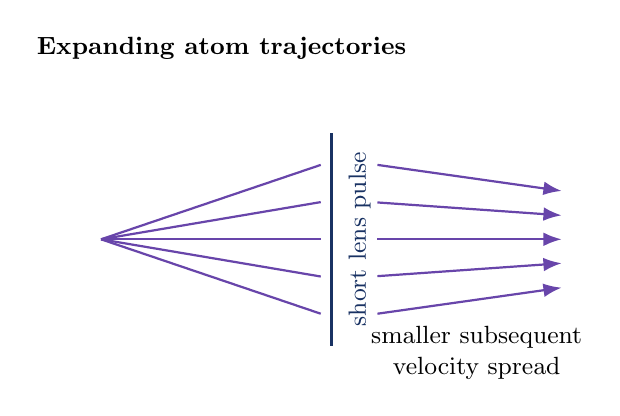
\begin{tikzpicture}[>=Latex,font=\small,scale=.9]
\node[font=\small\bfseries] at (1.7,2.7) {Expanding atom trajectories};
\foreach \y in {-0.7,-0.35,0,.35,.7}{\draw[thick,purple] (0,0) -- (3.1,{1.5*\y});}
\draw[deepblue,very thick] (3.25,-1.5)--(3.25,1.5);
\node[rotate=90,deepblue] at (3.65,0) {short lens pulse};
\foreach \y in {-1.05,-.52,0,.52,1.05}{\draw[->,thick,purple] (3.9,\y)--(6.5,{.65*\y});}
\node[align=center] at (5.3,-1.6) {smaller subsequent\\velocity spread};
\end{tikzpicture}\end{center}

\section{Imaging: what can a CCD or CMOS camera actually see?}
\subsection{Absorption imaging}
A probe laser passes through the atom cloud. In a simplified weak-saturation model, optical depth is related to column density by
\begin{equation}\mathrm{OD}(x,y)=\ln\!\frac{I_{\rm ref}(x,y)}{I_{\rm atoms}(x,y)}\simeq\sigma_{\rm eff}\int n(x,y,z)\dd z.\end{equation}
The camera records a line-of-sight integral, not the local three-dimensional wavefunction. In real work, finite saturation, detuning, polarization, optical pumping, aberrations and shot noise must be calibrated.

\subsection{Momentum distributions from time-of-flight}
For free ballistic motion at sufficiently long times and where interactions are negligible, position approximately maps to initial momentum, $\mathbf r\simeq\mathbf p t/M$. Thus the expanded density contains information about the initial momentum distribution. A BEC can give a narrow momentum component plus a broader thermal background. Fitting a narrow component must be justified against instrument resolution and interaction corrections.

\begin{example}[Optical depth to column density]
If $I_{\rm ref}/I_{\rm atoms}=e^{1.2}$, then OD $=1.2$. For an assumed calibrated effective cross section $\sigma_{\rm eff}=2.0\times10^{-13}$ m$^2$, the column density is $\tilde n=\mathrm{OD}/\sigma_{\rm eff}=6.0\times10^{12}$ atoms/m$^2$. The cross section here is an illustrative calibrated input, not a universal Rb-87 constant.
\end{example}

\section{Atomic interferometers as phase sensors}
A three-pulse light-pulse interferometer can act as a beam splitter, mirror and recombiner for atomic momentum states. In a standard ideal Mach--Zehnder-type geometry the acceleration-dependent phase is
\begin{equation}\boxed{\Delta\phi\simeq\mathbf k_{\rm eff}\cdot\mathbf a\,T^2+\phi_{\rm laser},}\end{equation}
where $T$ is pulse spacing, $\mathbf k_{\rm eff}$ is an effective wavevector and $\phi_{\rm laser}$ collects laser phase terms. Gravity gradients, finite pulses, rotations, wavefront errors, atom--atom interactions and initial conditions modify the response. A long cloud free-expansion time does \emph{not} automatically equal a demonstrated interferometer pulse spacing of the same duration.

\begin{example}[Acceleration sensitivity scaling]
For identical pulse geometry and $\mathbf k_{\rm eff}$, increasing $T$ from $1$ s to $2$ s multiplies an acceleration-induced phase by $4$. Increasing $T$ from $1$ to $7$ s would multiply it by $49$ \emph{if} a functioning interferometer supported that pulse spacing. This is a sensitivity-scaling illustration, not a claim about the Tiangong experiment.
\end{example}

\begin{example}[Order of magnitude of a gravity phase]
For counterpropagating Raman beams of wavelength $780$ nm, $k_{\rm eff}\approx4\pi/\lambda\simeq1.61\times10^7$ m$^{-1}$. A small acceleration $a=10^{-8}$ m/s$^2$ over $T=1$ s generates a phase $\Delta\phi\simeq0.161$ rad under the ideal model. State preparation, detection noise and systematic biases determine actual sensitivity.
\end{example}

\section{The November 2026 Tiangong experiment: what was measured?}
Xiong and collaborators reported a Bose--Einstein condensate produced in an optical dipole trap aboard China's space station, containing approximately $2.0\times10^4$ atoms. The abstract reports a seven-second free expansion and an equivalent expansion temperature $9.7^{+3.2}_{-2.7}$ pK, compared with a preceding $38$-pK benchmark and two-second expansion. The authors emphasize access to long free-evolution times for quantum simulation and precision measurement. The Chinese Academy of Sciences explicitly clarifies that this is the expansion-energy equivalent temperature, not the temperature of surrounding equipment.

\subsection{What can and cannot be inferred from the reported abstract}
The published abstract establishes condensate production, nominal atom count, seven-second free evolution and reported equivalent temperature. Those statements alone do not specify a full three-axis fit protocol, trap frequencies, initial widths, temperature anisotropy or the microscopic correlation function. Therefore this chapter deliberately does not invent an experimental dataset, a specific imaging fit, or an achieved interferometric gravity sensitivity.

\begin{center}\begin{tabularx}{\linewidth}{>{\bfseries}p{.36\linewidth}X}\toprule
Reported & $2.0\times10^4$ atoms; optical-dipole-trap BEC; $7.0$ s free expansion; $9.7^{+3.2}_{-2.7}$ pK equivalent expansion temperature.\\\midrule
Physical meaning & The cloud's low expansion energy permits a long, slowly spreading matter-wave measurement window.\\\midrule
Not established by those figures alone & Exact equilibrium entropy or thermodynamic temperature; interferometer sensitivity; raw widths and covariance; phase-coherence measurement.\\\bottomrule\end{tabularx}\end{center}

\section{Further worked numerical problems}
\begin{example}[Expansion temperature and energy]
At $9.7$ pK, $\kb T_{\rm eq}=1.339\times10^{-34}$ J $\simeq8.36\times10^{-16}$ eV. The notation specifies an energy scale; it does not require that atoms obey an equilibrium Maxwellian distribution.
\end{example}

\begin{example}[Effect of reducing velocity spread]
With zero initial covariance and a sufficiently long flight, $\sigma_x\simeq\sigma_vt$. Reducing the rms velocity from $100$ to $25\,\mu$m/s changes the seven-second expansion contribution from $700$ to $175\,\mu$m, a factor of four. The equivalent one-dimensional energy scale is reduced by $4^2=16$.
\end{example}

\begin{example}[Thermal wavelength as a contrast, not an in-situ measurement]
The usual equilibrium thermal wavelength is $\lambda_{\rm th}=h/\sqrt{2\pi M\kb T}$. For Rb-87 at $T=100$ nK it is approximately $0.59\,\mu$m. Formally inserting $10$ pK gives approximately $59\,\mu$m, but the latter is an energy-to-length conversion and is \emph{not} the experimentally measured Tiangong wavelength, because $T_{\rm eq}$ is based on expansion energy.
\end{example}

\section{Misconceptions and their precise corrections}
\begin{enumerate}[leftmargin=*,itemsep=4pt]
\item \textbf{``All electrons share a single orbital.''} No. The overlapping motional orbital describes complete atoms; electronic orbitals remain internal atomic degrees of freedom in the dilute-gas picture.
\item \textbf{``One matter wave means one 20,000-atom particle.''} No. A bosonic many-body state still contains $N$ atomic coordinates or, in Fock space, $N$ atoms occupying a mode.
\item \textbf{``A narrow image proves an equilibrium temperature of 10 pK.''} No. Expansion can reflect mean-field energy, quantum dispersion, correlations and collimation; the reported value is an equivalent expansion temperature.
\item \textbf{``Random fringe positions imply no coherence.''} Not necessarily. Independent condensates can have random relative phases from shot to shot while individual shots show interference.
\item \textbf{``No fringes means a normal gas.''} Not necessarily. Geometry, imbalance, finite resolution, projection and averaging can suppress visibility.
\item \textbf{``Seven-second expansion means a seven-second interferometer was operated.''} No. Free expansion provides an opportunity for interferometry but is not itself demonstration of a particular coherent beam-splitting sequence.
\end{enumerate}

\section{Exercises with concise answers}
\begin{enumerate}[leftmargin=*,itemsep=5pt]
\item Show that two equal-density modes have $\mathcal V=|g_{AB}^{(1)}|$ in an ideal two-mode model. \emph{Answer:} insert their mutual complex degree of coherence into the cross term of Eq.~\eqref{eq:interference}.
\item Find the fringe spacing for Rb-87 with $d=40\,\mu$m, $t=50$ ms. \emph{Answer:} $5.74\,\mu$m.
\item Determine $\sigma_v$ associated with $T_{\rm eq}=38$ pK using $M\sigma_v^2=\kb T_{\rm eq}$. \emph{Answer:} $60.3\,\mu$m/s.
\item Derive the free variance identity Eq.~\eqref{eq:variance}. \emph{Answer:} square $x(t)=x(0)+p(0)t/M$ using the symmetrized covariance.
\item Why does a vortex have a low-density core? \emph{Answer:} a nonzero winding phase produces divergent $|\nabla\theta|$ near $r=0$ unless the order-parameter amplitude tends to zero.
\item State two conditions where the Maxwellian width fit fails. \emph{Answer:} strong mean-field expansion and nonzero initial position--momentum covariance; others include anisotropic or nonthermal momentum distributions.
\end{enumerate}

\section{References and provenance}
\begin{enumerate}[leftmargin=*,itemsep=3pt]
\item W. Xiong, T. Li, S. Jin \emph{et al.}, ``Quantum gases below 10 picokelvin in space,'' \emph{Science} (5 November 2026), article eaea5324, DOI: \href{https://doi.org/10.1126/science.aea5324}{10.1126/science.aea5324}.
\item Chinese Academy of Sciences, ``China's Space Station Sets New Atomic Cooling Record,'' 6 November 2026, \href{https://english.cas.cn/newsroom/cas-in-media/202611/t20261106_1213502.shtml}{CAS news release}.
\item C. J. Pethick and H. Smith, \emph{Bose--Einstein Condensation in Dilute Gases}, Cambridge University Press.
\item L. Pitaevskii and S. Stringari, \emph{Bose--Einstein Condensation and Superfluidity}, Oxford University Press.
\item M. H. Anderson \emph{et al.}, ``Observation of Bose--Einstein condensation in a dilute atomic vapor,'' \emph{Science} \textbf{269} (1995), 198--201.
\item M. R. Andrews \emph{et al.}, ``Observation of interference between two Bose condensates,'' \emph{Science} \textbf{275} (1997), 637--641.
\item M. Kasevich and S. Chu, ``Atomic interferometry using stimulated Raman transitions,'' \emph{Physical Review Letters} \textbf{67} (1991), 181--184.
\item O. Penrose and L. Onsager, ``Bose--Einstein condensation and liquid helium,'' \emph{Physical Review} \textbf{104} (1956), 576--584.
\end{enumerate}

\clearpage
\section*{Supplementary Sections to Chapter II: deeper explanations (original chapter preserved)}
\addcontentsline{toc}{section}{Supplementary Sections to Chapter II}
\subsection*{II-A. Visibility is not identical to condensate fraction}
For two waves with intensities $I_A,I_B$ and degree of first-order coherence $|g^{(1)}|$, the fringe visibility (under the standard phase-stable interference arrangement) is
\begin{equation}V=\frac{I_{\max}-I_{\min}}{I_{\max}+I_{\min}}=\frac{2\sqrt{I_AI_B}}{I_A+I_B}|g^{(1)}|.\end{equation}
Balanced intensities give $V=|g^{(1)}|$, but unequal intensities reduce $V$ even for perfectly coherent fields. Conversely, a single-shot fringe pattern can arise between two independently prepared condensates with a random relative phase; averaging without phase alignment can wash the fringes out. Hence one must specify measurement protocol, ensemble, and phase reference when interpreting coherence.
\begin{example}[Visibility calculation]
With $I_A=9I_0$, $I_B=I_0$, and $|g^{(1)}|=0.8$, the predicted visibility is $V=2(3)/(10)\times0.8=0.48$, not $0.8$. Unequal envelopes matter.
\end{example}
\subsection*{II-B. The exact variance evolution and covariance}
For free motion $\hat x(t)=\hat x(0)+t\hat p(0)/M$. Therefore
\begin{equation}
\sigma_x^2(t)=\sigma_x^2(0)+\frac tM\langle\{\Delta x,\Delta p\}\rangle_0+\frac{t^2}{M^2}\sigma_p^2(0).
\end{equation}
A nonzero initial position--momentum covariance produces an intermediate-time focusing or defocusing contribution. In delta-kick collimation, lensing changes this covariance and reduces the far-field divergence. Reporting a single expansion slope without specifying a fit model may not uniquely identify a thermodynamic temperature.
\subsection*{II-C. Gaussian minimum uncertainty and expansion}
Start with $\psi(x,0)=(2\pi\sigma_0^2)^{-1/4}\exp[-x^2/(4\sigma_0^2)]$, where $\sigma_x(0)=\sigma_0$. For a minimum-uncertainty packet $\sigma_p(0)=\hbar/(2\sigma_0)$ and vanishing covariance, so
\begin{equation}\sigma_x(t)=\sqrt{\sigma_0^2+\left(\frac{\hbar t}{2M\sigma_0}\right)^2}.\end{equation}
This expansion persists even at zero thermodynamic temperature: it is quantum dispersion, not residual thermal agitation.
\begin{example}[A freely expanding atomic packet]
For $^{87}$Rb with $\sigma_0=10\,\mu$m and $t=1\,$s, the quantum-dispersion length $\hbar t/(2M\sigma_0)$ is about $36.5\,\mu$m, giving $\sigma_x(t)\simeq37.9\,\mu$m. A ground-state packet is not motionless.
\end{example}
\subsection*{II-D. What absorption imaging measures}
A resonant probe of initial intensity $I_0(x,y)$ traverses a cloud of column density $\widetilde n(x,y)=\int n(x,y,z)\,dz$. In the weak, unsaturated idealization, Beer--Lambert attenuation gives $I/I_0=\exp[-\sigma_{\rm abs}\widetilde n]$ and hence $\widetilde n=\ln(I_0/I)/\sigma_{\rm abs}$. Real experiments require corrections for saturation, detuning, polarization, imaging point-spread function and finite exposure. A density photograph does not directly show complex phase; interferometric preparation is needed for phase-sensitive information.
\subsection*{II-E. Why the Tiangong number is an equivalent temperature}
The reported $9.7^{+3.2}_{-2.7}\,$pK figure refers to an expansion-energy scale inferred from the prepared cloud, not a thermometer reading of the station or an assertion that the system is a conventional Maxwell--Boltzmann gas at that temperature. A one-dimensional convention $k_BT_{\rm eq}=M\sigma_v^2$ is useful only after the velocity measure and any contributions from interactions and wave-packet spreading have been specified. The reported seven-second expansion time by itself is not an interferometer interrogation time.

\end{document}
